% IPS PhD thesis template for LaTeX
% Erik Zupani�, Andreja Er�te

\documentclass[a4paper,11pt,twoside,final,openany]{book}  % fleqn enables left justification of equations in combination with \setlength{\mathindent}{1cm}
\usepackage[slovene,english]{babel}
\usepackage[T1]{fontenc}
\usepackage{mathptmx} % Uses font family: Times Roman
\usepackage{ae,aecompl}
\usepackage[latin2]{inputenc}
\usepackage{amsmath}
\usepackage{amssymb,mathrsfs}   % for \mathscr
%\setlength{\mathindent}{1cm}    % sets indentation of equations
\usepackage{graphicx}
\usepackage{url}
\usepackage{psfrag}
\usepackage{units}
\usepackage{fancyhdr}
\usepackage{setspace}
\usepackage[small]{caption}
\usepackage[top=2.2cm, bottom=2.5cm, left=2.5cm, right=2.5cm, bindingoffset=0.7cm]{geometry}
\usepackage{cite}
\usepackage{subfigure}
\usepackage{fixltx2e}   % Enables commands \textsuperscript and \textsubscript
\usepackage[nottoc,numbib]{tocbibind} % bibliography numbered

%% Tables
\usepackage[table]{xcolor}  % enables color cellc in tables
\usepackage{hhline}         % makes black lines when color cells are used (because \hline does not work)

%% Algorithms - float environment for custom Algorithms defined lower in the template: myalgorithm
% In this case, program package is selected and program environment is used for algorithms as subfloat in myalgortihm floats
\usepackage{program}

\usepackage{titlesec}
\usepackage{chngcntr}
\usepackage{titletoc}
\usepackage[subfigure]{tocloft} %manipulates contents lists
\usepackage{appendix}
\usepackage{float}

\usepackage[dvipdfm,colorlinks=true,       % false: boxed links; true: colored links
    linkcolor=black,          % color of internal links
    citecolor=black,        % color of links to bibliography
    filecolor=black,      % color of file links
    urlcolor=black           % color of external links
]{hyperref} %package for inputing urls and other links


%% Chapter titles and fonts
    %\usepackage{titlesec}
\titleformat{\chapter}[hang]{\normalfont\LARGE\bfseries}{\thechapter}{1em}{}
\titlespacing{\chapter}{0pt}{0pt}{35mm}
\addto\captionsenglish{\renewcommand\chaptername{}}   %remove chapter X
    %\usepackage{chngcntr}
\counterwithout{figure}{chapter}    %correct counting of figures - ips template style
\counterwithout{table}{chapter}     %correct counting of tables - ips template style
\counterwithout{equation}{chapter}  %correct counting of equations - ips template style

    %\usepackage{titletoc}
\titleformat{\chapter}[hang]{\normalfont\LARGE\bfseries}{\thechapter}{1em}{}
\titlespacing{\chapter}{0pt}{0pt}{35mm}
    %\usepackage[subfigure]{tocloft} %manipulates contents lists
\renewcommand{\cfttoctitlefont}{\LARGE\bfseries}
\setlength{\cftaftertoctitleskip}{35mm}
\renewcommand{\cftlottitlefont}{\LARGE\bfseries}
\setlength{\cftafterlottitleskip}{35mm}
\renewcommand{\cftloftitlefont}{\LARGE\bfseries}
\setlength{\cftafterloftitleskip}{35mm}
\renewcommand{\cfttabpresnum}{\tablename\ } %put the name before the number in the listoftables (lot)
\renewcommand{\cftfigpresnum}{\figurename\ } %put the name before the number in the listoffigures (lof)
\renewcommand{\cftfigaftersnum}{:} %put : after the number in the listoffigures
\renewcommand{\cfttabaftersnum}{:} %put : after the number in the listoftables
\setlength{\cfttabnumwidth}{5em} %space for the name before number in the listoftables
\setlength{\cftfignumwidth}{5em} %space for the name before number in the listoffigures
\setlength{\cftbeforefigskip}{0em} %changing the space between entries in the lof
\setlength{\cftbeforetabskip}{0em} %changing the space between entries in the lot

\setcounter{tocdepth}{9}    % shows numbers of subsections in toc
\setcounter{secnumdepth}{9} % numbers all sub(-sub)sections

%%
\renewcommand\citeleft{[}
\renewcommand\citeright{]}

\graphicspath{{images/}}

\makeatletter

%% myalgorithm float (used for writing algorithms) - definitions
%\usepackage{float}

%%
\newcommand\floatc@simplerule[2]{{\@fs@cfont #1 #2}\par}
\newcommand\fs@simplerule{\def\@fs@cfont{\bfseries}\let\@fs@capt\floatc@simplerule
  \def\@fs@pre{\hrule height0pt depth0pt \kern4pt}%
  \def\@fs@post{\kern4pt\hrule height0.1mm depth0pt \kern4pt \relax}%
  \def\@fs@mid{\kern8pt}%
  \let\@fs@iftopcapt\iftrue}

\floatstyle{simplerule}
\newfloat{myalgorithm}{thp}{lob}[chapter]
\floatname{myalgorithm}{Algorithm}
%\listof{myalgorithm}{Index of algorithms}
\counterwithout{myalgorithm}{chapter} %correct counting of algorithms - ips template style
%%
\newcommand{\listmyalgorithmname}{Index of Algorithms} %define the name for the list of algorithms (loa)
\newlistof{myalgorithms}{loa}{\listmyalgorithmname} %make newlistof
%\renewcommand{\cftmyalgorithmtitlefont}{\Large\bfseries}
%\setlength{\cftaftermyalgorithmtitleskip}{35mm}
%\setlength{\cftmyalgorithmsnumwidth}{5em} %space for the name before number in the listofalgorithms (loa)
%\setlength{\cftmybeforealgorithmsskip}{0em} %changing the space between entries in the loa


\newcommand{\HRule}{\rule{\linewidth}{0.1mm}} % defines line used in the example

\begin{document}

% *******************************************
%           First page (title page)
% *******************************************
%
% This page uses modified margins

\newgeometry{margin=2cm, bindingoffset=0.7cm}

\thispagestyle{empty}
\begin{flushright}
\noindent{\huge{\textbf{TITLE OF DISSERTATION}}}   % Insert: title of dissertation

    \vspace{3cm}

\noindent{\LARGE{Name and Surname of the Author}}  % Insert: name and surname of the author
\end{flushright}
\clearpage

%
% *******************************************
%

% *******************************************
%        Second page - information
% *******************************************
%
% This page uses modified margins

\newgeometry{margin=2cm, bindingoffset=1.2cm}

\thispagestyle{empty}

    \textnormal{ }\\ % empty line
    \textnormal{ }\\ % empty line
\vspace{2.1cm}

\noindent\textbf{Doctoral Dissertation}

\noindent\textbf{Jo\v{z}ef Stefan International Postgraduate School}

\noindent\textbf{Ljubljana, Slovenia, Month Year}   % Insert: month and year

\vspace{1.6cm}

\noindent\textbf{Evaluation Board:}\\   % Insert data about board members into lines below
\vspace{-2mm}
\begin{spacing}{1.35}
\noindent{\textit{Name and  surname of board member with the title, Chairman, institution and address}}\\
\noindent{\textit{Name and  surname of board member with the title, Member, institution and address}}\\
\noindent{\textit{Name and  surname of board member with the title, Member, institution and address}}
\end{spacing}

\clearpage

%
% *******************************************
%

% *******************************************
%        Third page - title page
% *******************************************
%
% This page uses modified margins

\newgeometry{margin=2cm, bindingoffset=1.2cm}

\thispagestyle{empty}

% IPS symbol (inserted as figure)
%
\vspace{-.5cm}
\begin{figure}[t]

\includegraphics[width=16cm]{header.eps}
\end{figure}

\vspace{4.2cm}
\textnormal{ }\\ % empty line

\noindent{\LARGE{Name and Surname of the Author}}\\ % Insert: name and surname of the author

\vspace{1.4cm}

\noindent{\huge{\textbf{TITLE OF DISSERTATION}}}\\   % Insert: title of dissertation in English

\vfill

\noindent{\LARGE{\textbf{Doctoral Dissertation}}}\\

\vfill

\noindent{\huge{\textbf{NASLOV DOKTORSKE DISERTA\-{CI}\-{JE}}}}\\   % Insert: title of dissertation in Slovene

\vfill

\noindent{\LARGE{\textbf{Doktorska disertacija}}}\\

\vfill

\noindent{\large{\textit{Supervisor}: Name and Surname with the title}}\\     % Insert: name and surname of supervisor with the title
    \textnormal{ }\\ % empty line
\noindent{\large{\textit{Co-Supervisor}: Name and Surname with the title}}\\     % Insert: name and surname of co-supervisor with the title
    \textnormal{ }\\ % empty line
    \textnormal{ }\\ % empty line
\noindent{\normalsize{Ljubljana, Slovenia, Month Year}}     % Insert: month and year

\vspace{1.4cm}

\clearpage

%
%
% *******************************************
% *******************************************
%
% *******************************************
%               Dissertation
% *******************************************
%
% From now on, document uses margins specified in the preamble
%
\restoregeometry

\thispagestyle{empty}

\renewcommand{\listfigurename}{Index of Figures}
\renewcommand{\listtablename}{Index of Tables}
\renewcommand{\contentsname}{Index}
\renewcommand{\bibname}{References}

\newcommand{\supers}[1]{\ensuremath{^{\textrm{#1}}}}
\newcommand{\subs}[1]{\ensuremath{_{\textrm{#1}}}}

\pagestyle{fancy}
\renewcommand{\chaptermark}[1]{\markboth{\thechapter.\ #1}{}}
%\renewcommand{\sectionmark}[1]{\markright {\thechapter.\ #1}}

\renewcommand{\headrulewidth}{0pt}
\renewcommand{\footrulewidth}{0pt}
\newcommand{\tim}{\fontfamily{tm}\fontseries{a}\fontsize{10}{12}\selectfont}

\fancyhf{}
\fancyhead[LE,RO]{\tim \thepage}
\fancyhead[LO,RE]{\tim \leftmark}

\fancypagestyle{plain}{
\fancyhf{}
\fancyhead[LE,RO]{\tim \thepage}
\renewcommand{\headrulewidth}{0pt}
\renewcommand{\footrulewidth}{0pt}}

\cleardoublepage
\newpage

\pagenumbering{Roman}
\pagestyle{fancy}
\setcounter{page}{5}

\tableofcontents

\cleardoublepage
\newpage

\addcontentsline{toc}{chapter}{Abstract} \chapter*{Abstract}

\noindent
First paragraph in current heading. First paragraph in current heading.
First paragraph in current heading. First paragraph in current heading.
First paragraph in current heading. First paragraph in current heading.
First paragraph in current heading. First paragraph in current heading.
First paragraph in current heading. 

Next paragraph in current heading. Next paragraph in current heading.
Next paragraph in current heading. Next paragraph in current heading.
Next paragraph in current heading. Next paragraph in current heading.
Next paragraph in current heading. Next paragraph in current heading.
Next paragraph in current heading. 

Next paragraph in current heading. Next paragraph in current heading.
Next paragraph in current heading. Next paragraph in current heading.
Next paragraph in current heading. Next paragraph in current heading.
Next paragraph in current heading. Next paragraph in current heading.
Next paragraph in current heading.


\thispagestyle{plain}
\clearpage
\newpage

\addcontentsline{toc}{chapter}{Povzetek} \chapter*{Povzetek}
\selectlanguage{slovene}

\noindent
Prvi odstavek teko�ega poglavja. Prvi odstavek teko�ega poglavja.
Prvi odstavek teko�ega poglavja. Prvi odstavek teko�ega poglavja.
Prvi odstavek teko�ega poglavja. Prvi odstavek teko�ega poglavja.
Prvi odstavek teko�ega poglavja. Prvi odstavek teko�ega poglavja.

Naslednji odstavek teko�ega poglavja. Naslednji odstavek teko�ega poglavja.
Naslednji odstavek teko�ega poglavja. Naslednji odstavek teko�ega poglavja.
Naslednji odstavek teko�ega poglavja. Naslednji odstavek teko�ega poglavja.
Naslednji odstavek teko�ega poglavja. Naslednji odstavek teko�ega poglavja.

Naslednji odstavek teko�ega poglavja. Naslednji odstavek teko�ega poglavja.
Naslednji odstavek teko�ega poglavja. Naslednji odstavek teko�ega poglavja.
Naslednji odstavek teko�ega poglavja. Naslednji odstavek teko�ega poglavja.
Naslednji odstavek teko�ega poglavja. Naslednji odstavek teko�ega poglavja.

\selectlanguage{english}

\thispagestyle{plain}
\clearpage
\newpage

\addcontentsline{toc}{chapter}{Abbreviations} \chapter*{Abbreviations}

% Abbreviations as a simple table
%%
\noindent
\begin{tabular}{ l p{3mm} p{1mm} l }
abbreviation one        & = & &     interpretation one      \\
abbreviation two        & = & &     interpretation two      \\
abbreviation three      & = & &     interpretation three    \\
abbreviation four       & = & &     interpretation four     \\
\end{tabular}
%%


%
% *************************************************************
%          LaTeX: Abbreviations as Nomenclature
% *************************************************************
%
% Add the next 4 lines somewhere in the preamble:
%
% \usepackage{nomencl}
% \setlength{\nomitemsep}{-\parsep}
% \makenomenclature
% \renewcommand{\nomname}{Abbrevations}
%
% Uncomment between %% for template:

%%
% \nomenclature{abbreviation1}{interpretation1}
% \nomenclature{abbreviation2}{interpretation2}
% \nomenclature{abbreviation3}{interpretation3}
% \nomenclature{abbreviation4}{interpretation4}
%
%\vspace{2cm}
%
%\printnomenclature[1.9cm]
%%

% IMPORTANT!
% For LaTeX a .nls file is needed:
% First, save this file, then LaTeX 00-disertation.tex two times.
% Use MakeIndex to create .nls file:
    % makeindex 00-disertation.nlo -s nomencl.ist -o 00-disertation.nls
% add manually in .nls  =\hspace{1.4cm} to make space between abbreviation and interpretation
%
% *************************************************************
%



\thispagestyle{fancy}
\markboth{Abbreviations}{}
\cleardoublepage
\newpage

\pagenumbering{arabic}
\pagestyle{fancy}
\renewcommand{\chaptermark}[1]{\markboth{#1}{}} % shows only chapter name in headder
%\renewcommand{\sectionmark}[1]{\markright{#1}{}}
\setcounter{page}{1}

\setlength{\subfigtopskip}{6mm} %vertical space between subfigures when \\ is used

\chapter{Introduction}

%
% ***************************************************************************
%             Formatting: Equations, Tables, Figures, Algorithms
% ***************************************************************************
%
% This section of the template contains some basic formatting instructions
% for formatting algorithms, equations, figures, and tables.
%
% In following chapters you will find some more examples.
%
%****************************************************************************
%

\noindent   % First paragraph has no indentation.
First paragraph in current heading. First paragraph in current heading.
First paragraph in current heading. First paragraph in current heading.
First paragraph in current heading. First paragraph in current heading.
First paragraph in current heading. First paragraph in current heading.
First paragraph in current heading.\cite{article-one}

%
% ********************************************
%         Formatting: Equations
% ********************************************
%
% A sample equation in equation environment:
%

Next paragraph in current heading. Next paragraph in current heading.
Next paragraph in current heading. Next paragraph in current heading.
Next paragraph in current heading. Next paragraph in current heading.
Next paragraph in current heading. Next paragraph in current heading.
Next paragraph in current heading.\cite{article-many,book-knownauthor,book-unknownauthor}

%%
\begin{equation}
\mathrm{\sigma ' = \varepsilon '' \varepsilon _{0} \omega}
\label{eq:sample}
\end{equation}
%%

Next paragraph in current heading. Next paragraph in current heading.
Next paragraph in current heading. Next paragraph in current heading.
Next paragraph in current heading. Next paragraph in current heading.
Next paragraph in current heading. Next paragraph in current heading.
Next paragraph in current heading.

%
% If fractions inside fractions are used, their font gets smaller until they have reached the \scriptstyle limit.
% In order to keep the size consistent, you can declare each fraction to use the display style instead, e.g. by using
% the \displaystyle command:
%

%%
\begin{equation}
x = a_0 + \frac{1}{\displaystyle a_1
+ \frac{1}{\displaystyle a_2
+ \frac{1}{\displaystyle a_3 + a_4}}}
\label{eq:fractions}
\end{equation}
%%

%
% For samples on arrays, matrices, breaking equations into several lines, etc., see
% http://en.wikibooks.org/wiki/LaTeX/Mathematics
%
% ********************************************
% ********************************************
%

Next paragraph in current heading. Next paragraph in current heading.
Next paragraph in current heading. Next paragraph in current heading.
Next paragraph in current heading. Next paragraph in current heading.
Next paragraph in current heading. Next paragraph in current heading.
Next paragraph in current heading.

% ********************************************
%         Formatting: Figures
% ********************************************
%
% Figures in figurename.eps format are supported in LaTeX.
% File subdirectory images contains figures used in the template.
%

%%
\begin{figure}[h!]
\centering
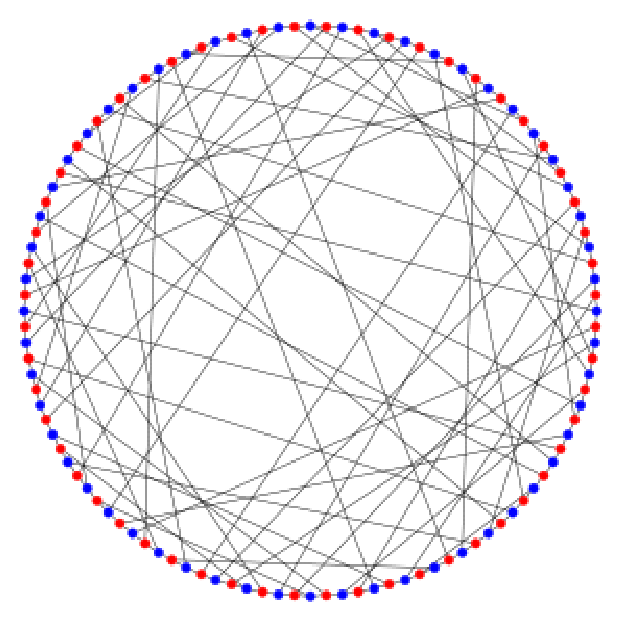
\includegraphics[width=6cm]{sample-1.eps}
\caption[Title]{\textit{Title.} Caption of this figure. Caption of this figure. Caption of this figure.
Caption of this figure. Caption of this figure. Caption of this figure. Caption of this figure. Caption of this figure.}
\label{fig:smiley}
\end{figure}
%%

%
% Using book documentclass, LaTeX automatically centers captions that fit into single line.
% This can be over-ruled by using justification:
% singlelinecheck=<bool>
% it switches the extra centering off by inserting false, no, off or 0 for <bool>
%

Next paragraph in current heading. Next paragraph in current heading.
Next paragraph in current heading. Next paragraph in current heading.
Next paragraph in current heading. Next paragraph in current heading.
Next paragraph in current heading. Next paragraph in current heading.
Next paragraph in current heading.

%

%%
\begin{figure}[h!]
\centering
\subfigure[]{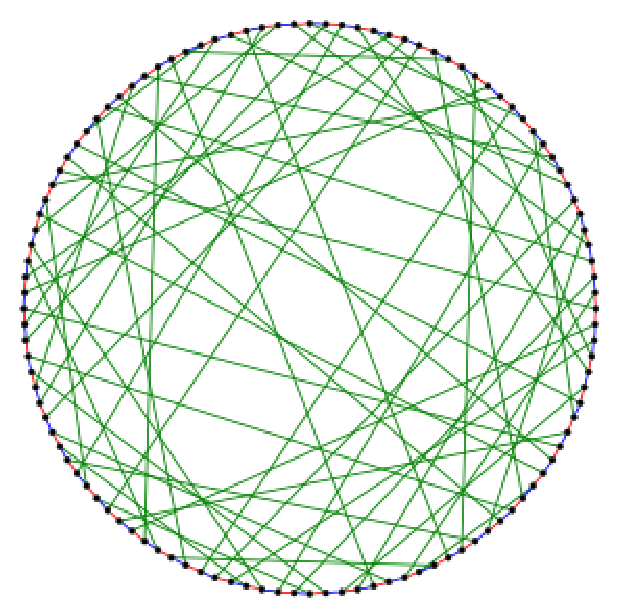
\includegraphics[width=5.5cm]{sample-2a.eps}}
\hspace{10mm}
\subfigure[]{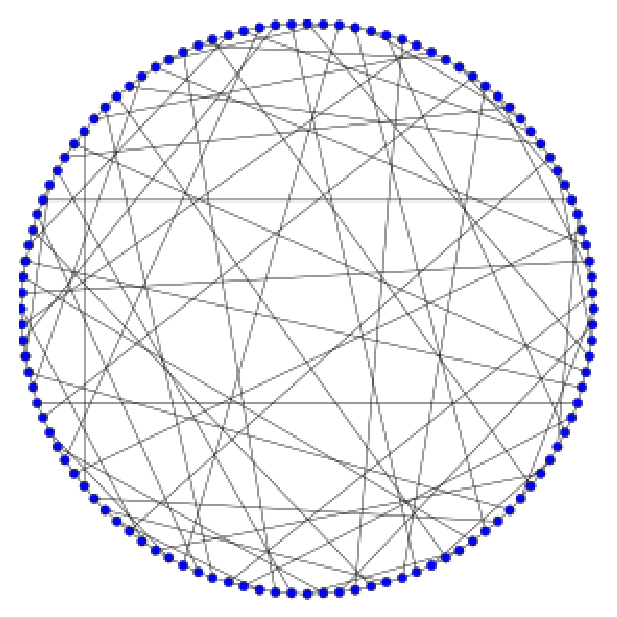
\includegraphics[width=5.7cm]{sample-2b.eps}}
\caption[Title]{\textit{Title.} Caption of this figure. Caption of this figure. Caption of this figure.
Caption of this figure. Caption of this figure. Caption of this figure. Caption of this figure. Caption of this figure.}
\label{fig:subfigures}
\end{figure}
%%

%
% ********************************************
% ********************************************
%

Next paragraph in current heading. Next paragraph in current heading.
Next paragraph in current heading. Next paragraph in current heading.
Next paragraph in current heading. Next paragraph in current heading.
Next paragraph in current heading. Next paragraph in current heading.
Next paragraph in current heading.

% ********************************************
%         Formatting: Tables
% ********************************************
%
% Sample table:
%

%%
\begin{table}[h!]
\captionof{table}[Title]{\textit{Title.} Caption of the table. Caption of the table. Caption of the table.
Caption of the table. Caption of the table. Caption of the table. Caption of the table. Caption of the table. Caption of the table.}
\label{tb:table}
\vspace{-5mm}
\begin{center}
\begin{tabular}{ p{3cm} p{11.4cm} }
\hhline{--}
\rowcolor[gray]{0.9} First line & \\ \hhline{--}
Text & This is the text \\
Text & This is the text \\
Text & This is the text \\
\hhline{--}
\end{tabular}
\end{center}
\end{table}
\vspace{-5mm}
%%

%
% In order to color the first row cell/-s, \rowcolor[gray]{0.9} is used.
% The word 'gray' here denotes the grayscale color scheme, not the color grey and `0.9' denotes how dark the grey is.
%
% The xcolor package provides the necessary commands to produce tables with alternate row colors, when loaded with the table option.
% The command \rowcolors{<starting row>}{<odd color>}{<even color>} has to be specified right before the tabular environment starts.
%
% For footnotes to work inside of tables, apply minipage environment before entering tabular environment.
%
% For more on tables, see
% http://en.wikibooks.org/wiki/LaTeX/Tables
%
% ********************************************
% ********************************************
%

Next paragraph in current heading. Next paragraph in current heading.
Next paragraph in current heading. Next paragraph in current heading.
Next paragraph in current heading. Next paragraph in current heading.
Next paragraph in current heading. Next paragraph in current heading.
Next paragraph in current heading.


Next paragraph in current heading. Next paragraph in current heading.
Next paragraph in current heading. Next paragraph in current heading.
Next paragraph in current heading. Next paragraph in current heading.
Next paragraph in current heading. Next paragraph in current heading.
Next paragraph in current heading.

Next paragraph in current heading. Next paragraph in current heading.
Next paragraph in current heading. Next paragraph in current heading.
Next paragraph in current heading. Next paragraph in current heading.
Next paragraph in current heading. Next paragraph in current heading.
Next paragraph in current heading.

Next paragraph in current heading. Next paragraph in current heading.
Next paragraph in current heading. Next paragraph in current heading.
Next paragraph in current heading. Next paragraph in current heading.
Next paragraph in current heading. Next paragraph in current heading.
Next paragraph in current heading.


Next paragraph in current heading. Next paragraph in current heading.
Next paragraph in current heading. Next paragraph in current heading.
Next paragraph in current heading. Next paragraph in current heading.
Next paragraph in current heading. Next paragraph in current heading.
Next paragraph in current heading.

Next paragraph in current heading. Next paragraph in current heading.
Next paragraph in current heading. Next paragraph in current heading.
Next paragraph in current heading. Next paragraph in current heading.
Next paragraph in current heading. Next paragraph in current heading.
Next paragraph in current heading.

%
% **********************************************
%         Formatting: Algorithms
% **********************************************
%
% In this case, a custom float is used for algorithms (as defined in preamble): myalgorithm
% Any environment can be then used for creation of algorithms when inserted inside the myalgorithm
% environment, e.g. algorithm, algorithmic, algorithm2e, program, verbatim,...
% Sample shows example of program float.

%%
\begin{myalgorithm}[h]
\centering
\caption[Title]{\textit{Title.} Caption of the algorithm. Caption of the algorithm.
Caption of the algorithm. Caption of the algorithm. Caption of the algorithm.
Caption of the algorithm.}
\HRule
\vspace{-9mm}
\begin{program}
\vspace{-2mm}
\mbox{A fast exponentiation procedure:}
\BEGIN %
  \FOR i:=1 \TO 10 \STEP 1 \DO
     |expt|(2,i); \\ |newline|() \OD %
\rcomment{This text will be set flush to the right margin}
\WHERE
\PROC |expt|(x,n) \BODY
          z:=1;
          \DO \IF n=0 \THEN \EXIT \FI;
             \DO \IF |odd|(n) \THEN \EXIT \FI;
\COMMENT{This is a comment statement};
                n:=n/2; x:=x*x \OD;
             \{ n>0 \};
             n:=n-1; z:=z*x \OD;
          |print|(z) \ENDPROC
\END
\end{program}
\vspace{-5mm}
\end{myalgorithm}
\vspace{-2mm}
%%

%
% In case you do not wish to use myalgorithm environment, make sure that the outcome of selected algorithm
% environment used looks as sample below (uncomment between %%). (in this case, also correct the Index of
% Algorithms accordingly).
%
% To see the sample, uncomment between %%

%% \newcommand{\HRule}{\rule{\linewidth}{0.1mm}} % defines line used in the example
%
%\vspace{4mm}
%\noindent{\small{Algorithm 1:                 % set separator as ':'
%\textit{Title of the Algorithm.}              % title of algorithm in italic text
%Caption of the Algorithm.                     % caption of algorithm in plain text on top
%}}
%
%\noindent\HRule
%
%\noindent This is the text.\\
%\noindent This is the text.\vspace{-3mm}\\
%\noindent\HRule
%\vspace{4mm}
%%

% For more on algorithms in algorithm environment, see
% http://en.wikibooks.org/wiki/LaTeX/Algorithms_and_Pseudocode
%
% For more on algorithms in algorithm2e environment, see
% http://www.tug.org/texlive/Contents/live/texmf-dist/doc/latex/algorithm2e/algorithm2e.pdf
%
% ********************************************
% ********************************************
%


Next paragraph in current heading. Next paragraph in current heading.
Next paragraph in current heading. Next paragraph in current heading.
Next paragraph in current heading. Next paragraph in current heading.
Next paragraph in current heading. Next paragraph in current heading.
Next paragraph in current heading.


\cleardoublepage

\chapter{Aims and hypothesis}

\noindent   % First paragraph has no indentation.
First paragraph in current heading. First paragraph in current heading.
First paragraph in current heading. First paragraph in current heading.
First paragraph in current heading. First paragraph in current heading.
First paragraph in current heading. First paragraph in current heading.
First paragraph in current heading.

Next paragraph in current heading. Next paragraph in current heading.
Next paragraph in current heading. Next paragraph in current heading.
Next paragraph in current heading. Next paragraph in current heading.
Next paragraph in current heading. Next paragraph in current heading.
Next paragraph in current heading.

\section{A section}

\noindent   % First paragraph has no indentation.
First paragraph in current heading. First paragraph in current heading.
First paragraph in current heading. First paragraph in current heading.
First paragraph in current heading. First paragraph in current heading.
First paragraph in current heading. First paragraph in current heading.
First paragraph in current heading.

Next paragraph in current heading. Next paragraph in current heading.
Next paragraph in current heading. Next paragraph in current heading.
Next paragraph in current heading. Next paragraph in current heading.
Next paragraph in current heading. Next paragraph in current heading.
Next paragraph in current heading.

Next paragraph in current heading. Next paragraph in current heading.
Next paragraph in current heading. Next paragraph in current heading.
Next paragraph in current heading. Next paragraph in current heading.
Next paragraph in current heading. Next paragraph in current heading.
Next paragraph in current heading.

Next paragraph in current heading. Next paragraph in current heading.
Next paragraph in current heading. Next paragraph in current heading.
Next paragraph in current heading. Next paragraph in current heading.
Next paragraph in current heading. Next paragraph in current heading.
Next paragraph in current heading.

% Example: Figure composed of three subfigures
\begin{figure}[h!]
\centering
\subfigure[]{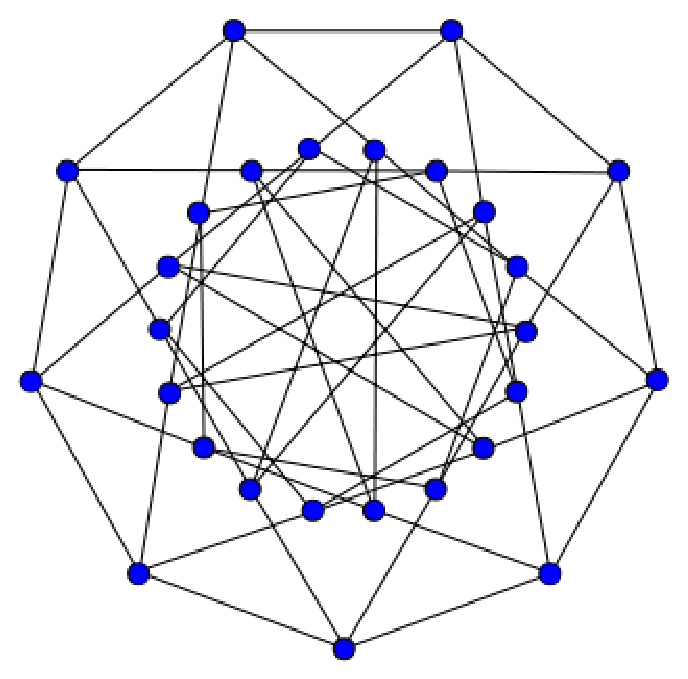
\includegraphics[width=5.1cm]{sample-3a.eps}}
\hspace{4mm}
\subfigure[]{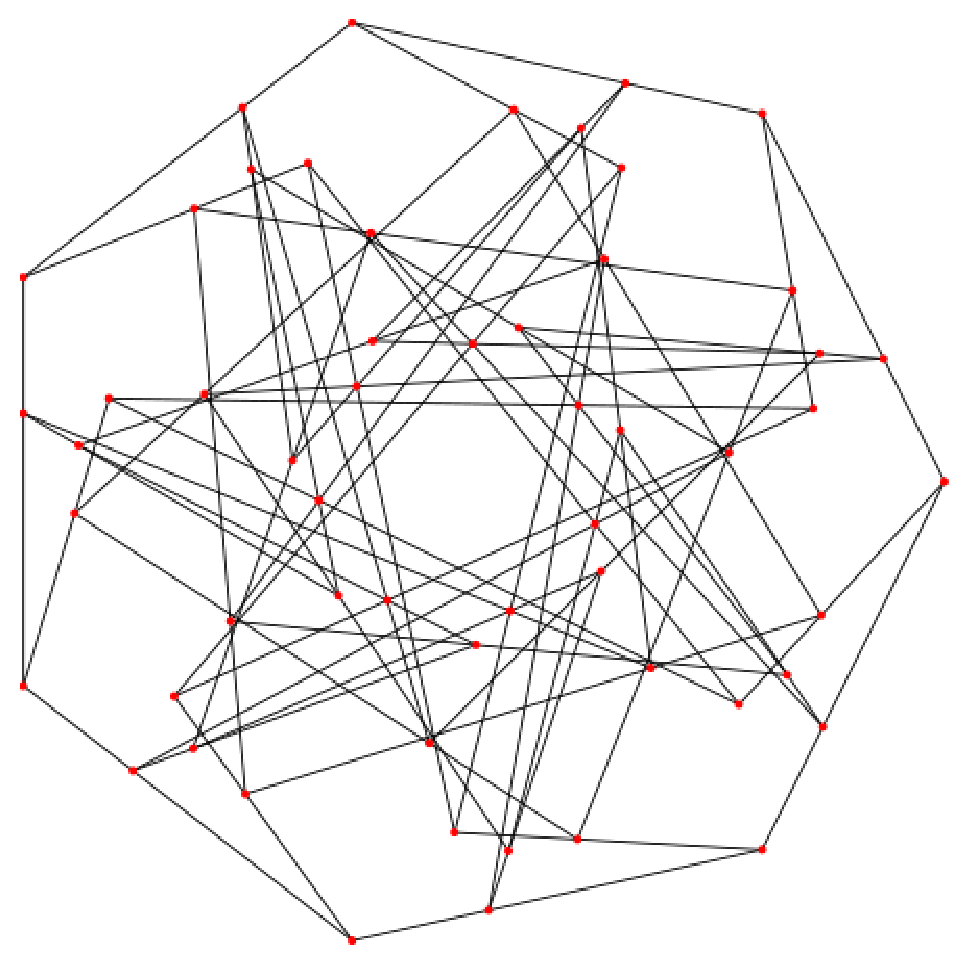
\includegraphics[width=5cm]{sample-3c.eps}}
\hspace{4mm}
\subfigure[]{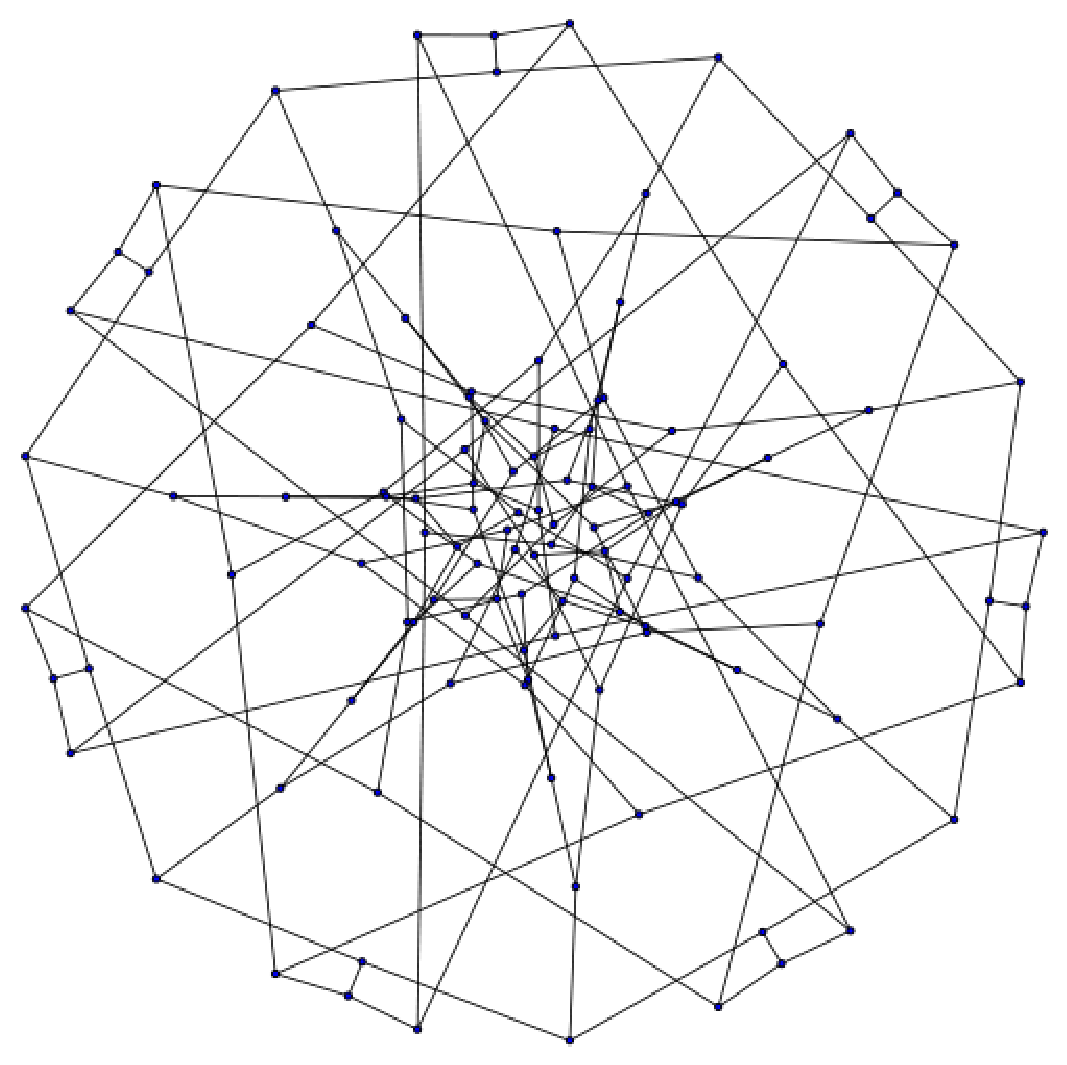
\includegraphics[width=5cm]{sample-3b.eps}}
\caption[Title.]{\textit{Title.} Caption of this figure. Caption of this figure. Caption of this figure.
Caption of this figure. Caption of this figure. Caption of this figure. Caption of this figure. Caption of this figure.}
\label{sts-resolution}
\end{figure}

Next paragraph in current heading. Next paragraph in current heading.
Next paragraph in current heading. Next paragraph in current heading.
Next paragraph in current heading. Next paragraph in current heading.
Next paragraph in current heading. Next paragraph in current heading.
Next paragraph in current heading.

    \subsection{A subsection}

\noindent   % First paragraph has no indentation.
First paragraph in current heading. First paragraph in current heading.
First paragraph in current heading. First paragraph in current heading.
First paragraph in current heading. First paragraph in current heading.
First paragraph in current heading. First paragraph in current heading.
First paragraph in current heading.

Next paragraph in current heading. Next paragraph in current heading.
Next paragraph in current heading. Next paragraph in current heading.
Next paragraph in current heading. Next paragraph in current heading.
Next paragraph in current heading. Next paragraph in current heading.
Next paragraph in current heading.

Next paragraph in current heading. Next paragraph in current heading.
Next paragraph in current heading. Next paragraph in current heading.
Next paragraph in current heading. Next paragraph in current heading.
Next paragraph in current heading. Next paragraph in current heading.
Next paragraph in current heading.


        \subsubsection{A subsubsection}

\noindent   % First paragraph has no indentation.
First paragraph in current heading. First paragraph in current heading.
First paragraph in current heading. First paragraph in current heading.
First paragraph in current heading. First paragraph in current heading.
First paragraph in current heading. First paragraph in current heading.
First paragraph in current heading.

Next paragraph in current heading. Next paragraph in current heading.
Next paragraph in current heading. Next paragraph in current heading.
Next paragraph in current heading. Next paragraph in current heading.
Next paragraph in current heading. Next paragraph in current heading.
Next paragraph in current heading.




\cleardoublepage

\include{03-Materials-and-Methods}
\cleardoublepage

\chapter{Results}

\noindent   % First paragraph has no indentation.
First paragraph in current heading. First paragraph in current heading.
First paragraph in current heading. First paragraph in current heading.
First paragraph in current heading. First paragraph in current heading.
First paragraph in current heading. First paragraph in current heading.
First paragraph in current heading.

Next paragraph in current heading. Next paragraph in current heading.
Next paragraph in current heading. Next paragraph in current heading.
Next paragraph in current heading. Next paragraph in current heading.
Next paragraph in current heading. Next paragraph in current heading.
Next paragraph in current heading.

\section{A section}

\noindent   % First paragraph has no indentation.
First paragraph in current heading. First paragraph in current heading.
First paragraph in current heading. First paragraph in current heading.
First paragraph in current heading. First paragraph in current heading.
First paragraph in current heading. First paragraph in current heading.
First paragraph in current heading.

Next paragraph in current heading. Next paragraph in current heading.
Next paragraph in current heading. Next paragraph in current heading.
Next paragraph in current heading. Next paragraph in current heading.
Next paragraph in current heading. Next paragraph in current heading.
Next paragraph in current heading.

    \subsection{A subsection}

\noindent   % First paragraph has no indentation.
First paragraph in current heading. First paragraph in current heading.
First paragraph in current heading. First paragraph in current heading.
First paragraph in current heading. First paragraph in current heading.
First paragraph in current heading. First paragraph in current heading.
First paragraph in current heading.

Next paragraph in current heading. Next paragraph in current heading.
Next paragraph in current heading. Next paragraph in current heading.
Next paragraph in current heading. Next paragraph in current heading.
Next paragraph in current heading. Next paragraph in current heading.
Next paragraph in current heading.

\section{A section}

\noindent   % First paragraph has no indentation.
First paragraph in current heading. First paragraph in current heading.
First paragraph in current heading. First paragraph in current heading.
First paragraph in current heading. First paragraph in current heading.
First paragraph in current heading. First paragraph in current heading.
First paragraph in current heading.

Next paragraph in current heading. Next paragraph in current heading.
Next paragraph in current heading. Next paragraph in current heading.
Next paragraph in current heading. Next paragraph in current heading.
Next paragraph in current heading. Next paragraph in current heading.
Next paragraph in current heading.


\cleardoublepage

\include{05-Discussion}
\cleardoublepage

\chapter{Conclusions}

\noindent   % First paragraph has no indentation.
First paragraph in current heading. First paragraph in current heading.
First paragraph in current heading. First paragraph in current heading.
First paragraph in current heading. First paragraph in current heading.
First paragraph in current heading. First paragraph in current heading.
First paragraph in current heading.

Next paragraph in current heading. Next paragraph in current heading.
Next paragraph in current heading. Next paragraph in current heading.
Next paragraph in current heading. Next paragraph in current heading.
Next paragraph in current heading. Next paragraph in current heading.
Next paragraph in current heading.





















\cleardoublepage

\chapter{Acknowledgements}

\noindent
These are the acknowledgments.
\cleardoublepage

\thispagestyle{plain}

% *********************************************
%               The Bibliography
% *********************************************
%
% For BibTex, style ''nature'' has been created (it is located in the root file directory).
% Uncomment between %% and comment between %%% to use BibTex for references.

%%
%\bibliographystyle{nature}
%\cleardoublepage
%\renewcommand{\bibname}{References}
%   \nocite{*}
%\bibliography{ref/references}
%%

% *********************************************
%
% For manual insert of references, write them in 00bib-References.tex file

%%%
\cleardoublepage
\renewcommand{\bibname}{References}
  \nocite{*}
\begin{thebibliography}{999}

% Article in a magazine
\bibitem{article-one}   Shapiro, B.
                        Expansion of a Bose-Einstein Condensate in the Presence of Disorder.
                        \textit{Physical Review Letters}
                        \textbf{99}, 060602 (2007).


\bibitem{article-many}  Grzybowska, K.; Grzybowski, A.; Ziolo, J; Rzoska, S. J.; Paluch, M.
                        Anomalous behaviour of secondary dielectric relaxation in polypropylene glycols.
                        \textit{Journal of Physics: Condensed Matter}
                        \textbf{19}, 376105 (2007).

% Books
    % Known author

\bibitem{book-knownauthor}      Goffer, Z.
                                \textit{Archaeological Chemistry: A Sourcebook on the Applications of Chemistry to Archaeology}
                                (John Wiley, New York, 1980).

    % If there is no known author, cite editor
\bibitem{book-unknownauthor}    Bandy, A. R. (ur.).
                                \textit{The Chemistry of the Atmosphere: Oxidants and Oxidation in the Earth's Atmosphere}
                                (Royal Society of Chemistry, Cambridge, 1995).

% Proceedings
\bibitem{proceeding}    Ponnambalam, M. J.
                        Electric Field Gradient in Aluminium due to Vacancy and Muon.
                        In: \textit{Proceedings of the XI\textsuperscript{th} International Symposium on NQR Spectroscopy.}
                        5-49 (Verlag der Zeitschrift f�r Naturfoeschung, T�bingen, 1991).

% Chapter in a book
\bibitem{chapter-book}  Sintak, Y.
                        Models and projections of energy use in the Soviet Union.
                        In: \textit{Steiner, T. (ed.) International energy economics.}
                        1-53 (Chapman and Hall, London, 1999).


% Article in a newspaper
\bibitem{newsapaper}    Blinc, R.
                        Uporabni "dvoli\v{c}ne\v{z}i": Magnetoelektriki.
                        \textit{Delo}
                        49/182, 16 (9.7.2007).

% Webpage
\bibitem{web}           Hildebrand, A. J.
                        \LaTeX tips: Bibliographies. \\
                        \url{http://www.math.uiuc.edu/~hildebr/tex/bibliographies.html}\\
                        (accessed: November 2011).


\end{thebibliography} 
%%%


% *********************************************
%

\newpage
\cleardoublepage
\renewcommand{\listfigurename}{Index of Figures} \listoffigures
\newpage

\cleardoublepage
\renewcommand{\listtablename}{Index of Tables} \listoftables
\newpage

\cleardoublepage
\addcontentsline{toc}{chapter}{Index of Algorithms}
\listof{myalgorithm}{Index of Algorithms}
\newpage

\newpage
\cleardoublepage


\appendix

%%
%To not show sections in TOC use new command \tocless (uncomment next two lines)
%\newcommand{\nocontentsline}[3]{}
%\newcommand{\tocless}[2]{\bgroup\let\addcontentsline=\nocontentsline#1{#2}\egroup}
%
%% Example:
%\tocless\section{hide}
%\tocless\subsection{subhide}
%%

\renewcommand*{\thechapter}{ }
\renewcommand*{\thesection}{\Alph{section}}
\chapter{Appendix}
\section{Appendix 1}
\noindent
List of publications related to this dissertation.

\cleardoublepage

\section{Appendix 2}
\noindent
This is another appendix.



\end{document}
